\documentclass[border=6pt,tikz]{standalone}
\usepackage{tikz}
\usepackage{amsmath,amssymb}
\usetikzlibrary{arrows.meta,positioning,fit,backgrounds,calc,shapes.geometric,decorations.pathreplacing,patterns}
\definecolor{ink}{HTML}{1B2430}
\definecolor{muted}{HTML}{6B7785}
\definecolor{accent}{HTML}{2F6FB5}
\definecolor{accent2}{HTML}{C1611F}
\definecolor{good}{HTML}{2E7D5B}
\definecolor{soft}{HTML}{EDF2F7}
\definecolor{soft2}{HTML}{FBEDE2}
\definecolor{soft3}{HTML}{E6F0E9}
\tikzset{
  box/.style={draw=ink,line width=.7pt,rounded corners=2pt,fill=soft,inner sep=4pt,align=center,font=\sffamily\small},
  boxa/.style={box,fill=soft2},
  boxb/.style={box,fill=soft3},
  plain/.style={align=center,font=\sffamily\small,text=ink},
  tiny/.style={align=center,font=\sffamily\scriptsize,text=muted},
  ar/.style={-{Stealth[length=2.4mm]},draw=ink,line width=.7pt},
  arm/.style={-{Stealth[length=2.4mm]},draw=muted,line width=.6pt,dashed},
  nd/.style={circle,draw=ink,line width=.7pt,fill=white,minimum size=7mm,inner sep=0pt,font=\sffamily\scriptsize},
  ndf/.style={nd,fill=soft},
  ndt/.style={nd,fill=soft2},
}

\begin{document}

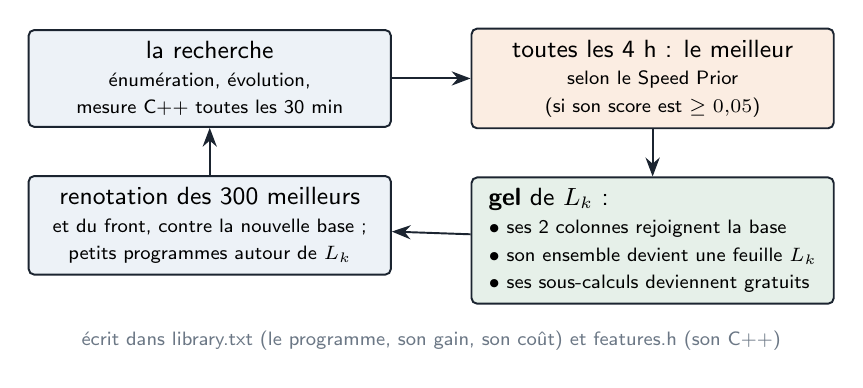
\begin{tikzpicture}[node distance=6mm and 10mm]
\node[box,minimum width=46mm] (search) {la recherche\\[-1pt]\scriptsize énumération, évolution,\\[-1pt]\scriptsize mesure C++ toutes les 30 min};
\node[boxa,right=of search,minimum width=46mm] (pick) {toutes les 4 h : le meilleur\\[-1pt]\scriptsize selon le Speed Prior\\[-1pt]\scriptsize (si son score est $\ge 0{,}05$)};
\node[boxb,below=of pick,minimum width=46mm,align=left] (freeze) {\textbf{gel} de $L_k$ :\\[-1pt]\scriptsize $\bullet$ ses 2 colonnes rejoignent la base\\[-1pt]\scriptsize $\bullet$ son ensemble devient une feuille $L_k$\\[-1pt]\scriptsize $\bullet$ ses sous-calculs deviennent gratuits};
\node[box,below=of search,minimum width=46mm] (rescore) {renotation des 300 meilleurs\\[-1pt]\scriptsize et du front, contre la nouvelle base ;\\[-1pt]\scriptsize petits programmes autour de $L_k$};
\draw[ar] (search) -- (pick);
\draw[ar] (pick) -- (freeze);
\draw[ar] (freeze) -- (rescore);
\draw[ar] (rescore) -- (search);
\node[plain,below=4mm of $(rescore.south)!0.5!(freeze.south)$,text=muted] {\scriptsize écrit dans library.txt (le programme, son gain, son coût) et features.h (son C++)};
\end{tikzpicture}
\end{document}
